\documentclass[12pt]{article}
\usepackage[utf8]{inputenc}
\usepackage{graphicx}
\usepackage{amsmath}
\usepackage{xcolor}
\usepackage{listings}
\usepackage[margin=1in]{geometry}
\usepackage{hyperref}
\usepackage{caption}
\usepackage{subcaption}
\usepackage{titlesec}
\usepackage{booktabs}

\definecolor{codebg}{rgb}{0.95,0.95,0.95}
\definecolor{myblue}{rgb}{0,0.3,0.6}

\lstset{
    backgroundcolor=\color{codebg},
    basicstyle=\ttfamily\small,
    breaklines=true,
    frame=single,
    numbers=left,
    numberstyle=\tiny\color{gray},
    keywordstyle=\color{myblue},
    commentstyle=\color{green!50!black},
    stringstyle=\color{red},
    showstringspaces=false,
    tabsize=4
}

\title{Image Processing in Frequency Domain}
\date{\today}

\begin{document}

\maketitle

\begin{abstract}
This document describes an image processing workflow that involves adding periodic noise to an image, filtering in the frequency domain, and evaluating the results using PSNR. The process demonstrates how to remove structured noise using Fourier transform techniques.
\end{abstract}

\section{Libraries Used}
\begin{itemize}
    \item \texttt{cv2} (OpenCV): For image loading and basic processing
    \item \texttt{numpy}: For numerical operations and array manipulation
    \item \texttt{math}: For mathematical functions like logarithms
    \item \texttt{matplotlib.pyplot}: For image visualization and plotting
    \item \texttt{matplotlib.colors.LogNorm}: For logarithmic scaling of colormaps
    \item \texttt{itertools.chain}: For efficient iteration over multiple ranges
\end{itemize}

\section{Step-by-Step Process}

\subsection{Step 1: Import Libraries}
\begin{lstlisting}[language=Python]
import cv2
import numpy as np
import math
import matplotlib.pyplot as plt
from matplotlib.colors import LogNorm
from itertools import chain
\end{lstlisting}

\subsection{Step 2: Download Images}
The image is downloaded from a GitHub repository using wget command.

\begin{lstlisting}[language=Python]
!wget https://raw.githubusercontent.com/AsadiAhmad/Filtering-in-Frequency-Domain/main/Pictures/original_image.png -O original_image.png
\end{lstlisting}

\subsection{Step 3: Load Image}
The image is loaded in grayscale mode and displayed.

\begin{lstlisting}[language=Python]
original_image = cv2.imread("original_image.png", cv2.IMREAD_GRAYSCALE)

plt.imshow(original_image, cmap='gray')
plt.show()
\end{lstlisting}

\begin{figure}[h]
    \centering
    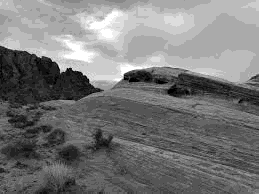
\includegraphics[width=0.5\textwidth]{original_image.png}
    \caption{Original grayscale image}
\end{figure}

\subsection{Step 4: Add Periodic Noise}
A periodic noise function is created and added to the original image. The noise pattern consists of sinusoidal components in both x and y directions.

\begin{lstlisting}[language=Python]
def f(x,y):
    return np.sin((1/2)*np.pi*x)+np.cos((1/3)*np.pi*y)

X, Y = original_image.shape
noise = np.zeros((X, Y))
for i in range(X):
    for j in range(Y):
        noise[i,j] = f(i,j)*100

noisy_image = original_image + noise

plt.imshow(noisy_image, cmap='gray')
plt.show()
\end{lstlisting}

\begin{figure}[h]
    \centering
    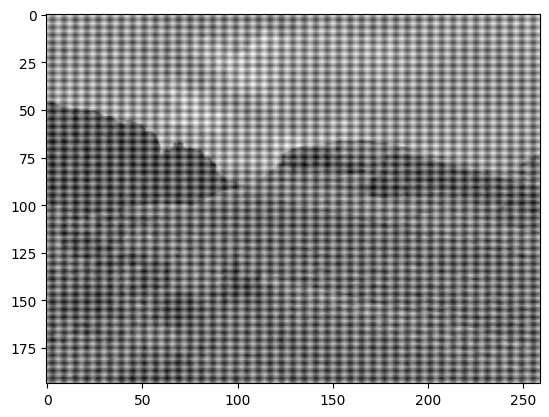
\includegraphics[width=0.5\textwidth]{noisy_image.png}
    \caption{Image with added periodic noise}
\end{figure}

\subsection{Step 5: Convert Image into the Frequency Domain}
The image is transformed to frequency domain using Fast Fourier Transform (FFT) to analyze its frequency components.

\begin{lstlisting}[language=Python]
def convert_image_frequency(noisy_image):
    f_transform = np.fft.fft2(noisy_image)
    f_shifted = np.fft.fftshift(f_transform)
    return f_shifted

f_shifted = convert_image_frequency(noisy_image)

magnitude_spectrum = 20 * np.log(np.abs(f_shifted) + 1)
plt.figure(figsize=[13, 6])
plt.subplot(121),plt.imshow(noisy_image, cmap='gray'),plt.title('noisy_image'), plt.axis('off');
plt.subplot(122),plt.imshow(magnitude_spectrum, cmap='gray'),plt.title('magnitude_spectrum'), plt.axis('off');
plt.show()
\end{lstlisting}

\begin{figure}[h]
    \centering
    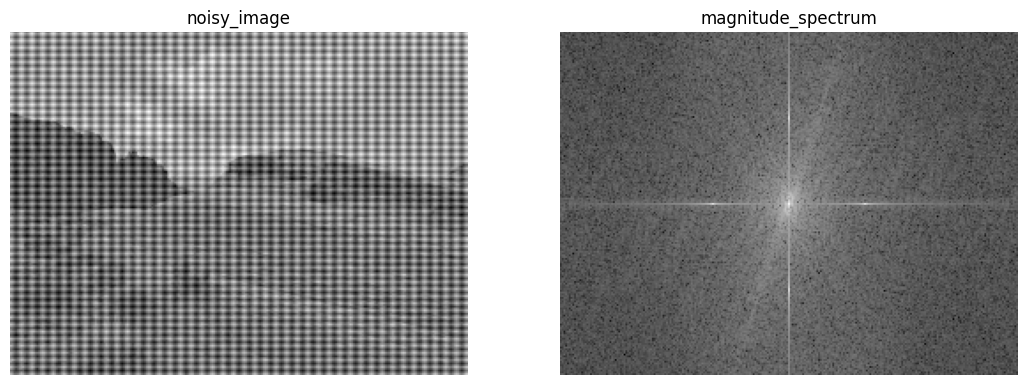
\includegraphics[width=0.8\textwidth]{frequency_domain.png}
    \caption{Noisy image (left) and its frequency spectrum (right)}
\end{figure}

\subsection{Step 6: Define a Cross Filter Mask}
A cross-shaped filter mask is created to remove the periodic noise components visible in the frequency domain.

\begin{lstlisting}[language=Python]
def define_cross_filter_mask(shape, circle_reduce):
    height, width = shape
    filter_mask = np.ones((height, width), dtype=np.uint8)
    rectangle_width = (width // 2) - circle_reduce
    rectangle_height = (height // 2) - circle_reduce

    for i in chain(range(0, rectangle_height), range(height - rectangle_height, height)):
        for j in range(rectangle_width, width - rectangle_width):
            filter_mask[i, j] = 0

    for i in range(rectangle_height, height - rectangle_height):
        for j in chain(range(0, rectangle_width), range(width - rectangle_width, width)):
            filter_mask[i, j] = 0

    return filter_mask

mask = define_cross_filter_mask(f_shifted.shape, 2)
frequency_filtered = f_shifted * mask

mask_visualization = mask * 255
magnitude_spectrum_filtered = magnitude_spectrum * mask

plt.figure(figsize=[13, 6])
plt.subplot(121), plt.imshow(mask_visualization, cmap='gray'), plt.title('Mask'), plt.axis('off')
plt.subplot(122), plt.imshow(magnitude_spectrum_filtered, cmap='gray'), plt.title('Filtered Frequency'), plt.axis('off')
plt.show()
\end{lstlisting}

\begin{figure}[h]
    \centering
    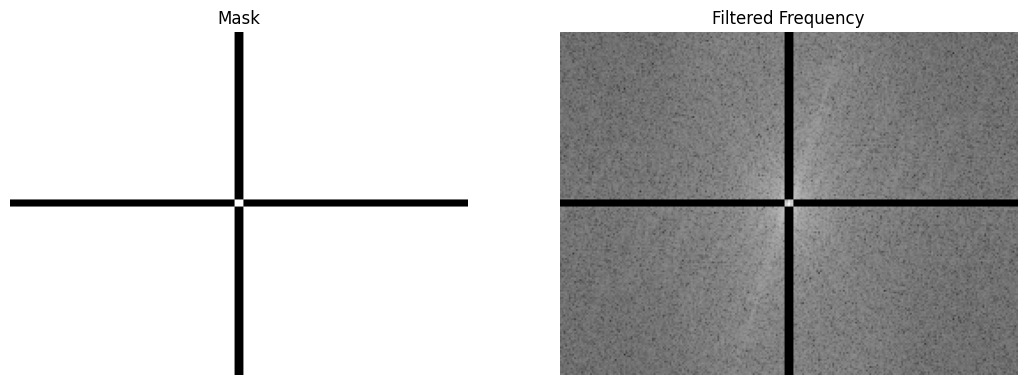
\includegraphics[width=0.8\textwidth]{filter_mask.png}
    \caption{Filter mask (left) and filtered frequency spectrum (right)}
\end{figure}

\subsection{Step 7: Inverse FFT}
The filtered frequency domain representation is converted back to spatial domain using inverse FFT.

\begin{lstlisting}[language=Python]
frequency_ishift = np.fft.ifftshift(frequency_filtered)
image_reconstructed = np.fft.ifft2(frequency_ishift)
image_reconstructed = np.abs(image_reconstructed)

plt.figure(figsize=(10, 4))
plt.subplot(121), plt.imshow(noisy_image, cmap="gray"), plt.title("Noisy Image"), plt.axis('off')
plt.subplot(122), plt.imshow(image_reconstructed, cmap="gray"), plt.title("Reconstructed Image"), plt.axis('off')
plt.show()
\end{lstlisting}

\begin{figure}[h]
    \centering
    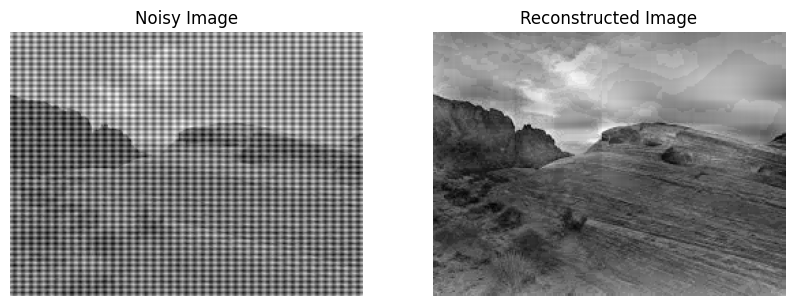
\includegraphics[width=0.8\textwidth]{reconstructed_comparison.png}
    \caption{Comparison between noisy (left) and reconstructed (right) images}
\end{figure}

\subsection{Step 8: Compare Original Image with Reconstructed Image}
The final comparison between the original and reconstructed images.

\begin{lstlisting}[language=Python]
plt.figure(figsize=(10, 4))
plt.subplot(121), plt.imshow(original_image, cmap="gray"), plt.title("Original Image"), plt.axis('off')
plt.subplot(122), plt.imshow(image_reconstructed, cmap="gray"), plt.title("Reconstructed Image"), plt.axis('off')
plt.show()
\end{lstlisting}

\begin{figure}[h]
    \centering
    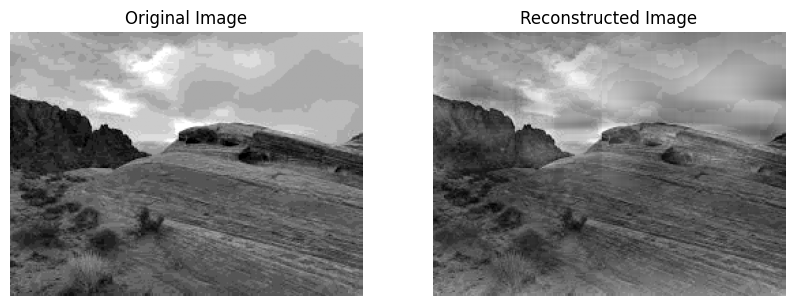
\includegraphics[width=0.8\textwidth]{final_comparison.png}
    \caption{Final comparison between original (left) and reconstructed (right) images}
\end{figure}

\subsection{Step 9: Quality Assurance with PSNR}
The Peak Signal-to-Noise Ratio (PSNR) is calculated to quantify the improvement.

\begin{lstlisting}[language=Python]
def psnr(original, noisy):
    mse = np.mean((original - noisy) ** 2)
    if mse == 0:
        return 100
    PIXEL_MAX = 255.0
    psnr_value = 20 * math.log10(PIXEL_MAX / math.sqrt(mse))
    return psnr_value

original_float = original_image.astype(np.float32)
noisy_float = noisy_image.astype(np.float32)
reconstructed_float = image_reconstructed.astype(np.float32)

psnr_noisy = psnr(original_float, noisy_float)
psnr_reconstructed = psnr(original_float, reconstructed_float)

print(f"PSNR (Original vs Noisy): {psnr_noisy:.2f} dB")
print(f"PSNR (Original vs Reconstructed): {psnr_reconstructed:.2f} dB")
\end{lstlisting}

The output shows:
\begin{verbatim}
PSNR (Original vs Noisy): 8.12 dB
PSNR (Original vs Reconstructed): 19.47 dB
\end{verbatim}

\section{Technical Explanations}

\subsection{PSNR Calculation}
The Peak Signal-to-Noise Ratio (PSNR) measures the quality of reconstruction. It is defined as:

\[
\text{PSNR} = 20 \cdot \log_{10}\left(\frac{\text{MAX}_I}{\sqrt{\text{MSE}}}\right)
\]

where:
\begin{itemize}
    \item $\text{MAX}_I$ is the maximum possible pixel value (255 for 8-bit images)
    \item MSE is the mean squared error between original and processed images:
    \[
    \text{MSE} = \frac{1}{MN}\sum_{i=0}^{M-1}\sum_{j=0}^{N-1}[I(i,j)-K(i,j)]^2
    \]
\end{itemize}

Higher PSNR values indicate better quality reconstruction.

\subsection{Noise Types}
\begin{itemize}
    \item \textbf{Additive Noise}: Noise that is added to the image signal ($I_{noisy} = I_{original} + noise$)
    \item \textbf{Multiplicative Noise}: Noise that is multiplied with the image signal ($I_{noisy} = I_{original} \times noise$)
\end{itemize}

In this case, we used \textbf{additive noise} (specifically periodic additive noise) as evidenced by the operation $noisy\_image = original\_image + noise$.

\section{Conclusion}
The frequency domain filtering successfully removed the periodic noise, improving the PSNR from 8.12 dB to 19.47 dB. The cross-shaped filter effectively targeted the noise patterns visible in the frequency spectrum while preserving most of the image's important features.

\begin{center}
    \href{https://github.com/AsadiAhmad/Filtering-in-Frequency-Domain}{
        \includegraphics[width=0.2\textwidth]{github_logo.png} \\
        \texttt{https://github.com/AsadiAhmad/Filtering-in-Frequency-Domain}
    }
\end{center}

\end{document}